\section{Results}

\subsection{Results Overview}

Despite only having the resources to apply our model to existing stops within the Spartanburg bus system, we obtained results that we believe are indicative of our model being a sound way to generally assess accessibility to services and amenities. We were able to apply the model in its full capacity to two existing bus routes: one in a very dense shopping district, and another in a more residential area. We were also able to apply a simplified version of the model - only considering the three services/amenities with the highest point value - to four additional stops. As a means of performing sensitivity analysis, we also applied this simplified version of the model to the two stops that received the full model application as well


\subsection{Full Model Application on Two Existing Bus Stops}

\begin{figure}[ht]
    \centering
    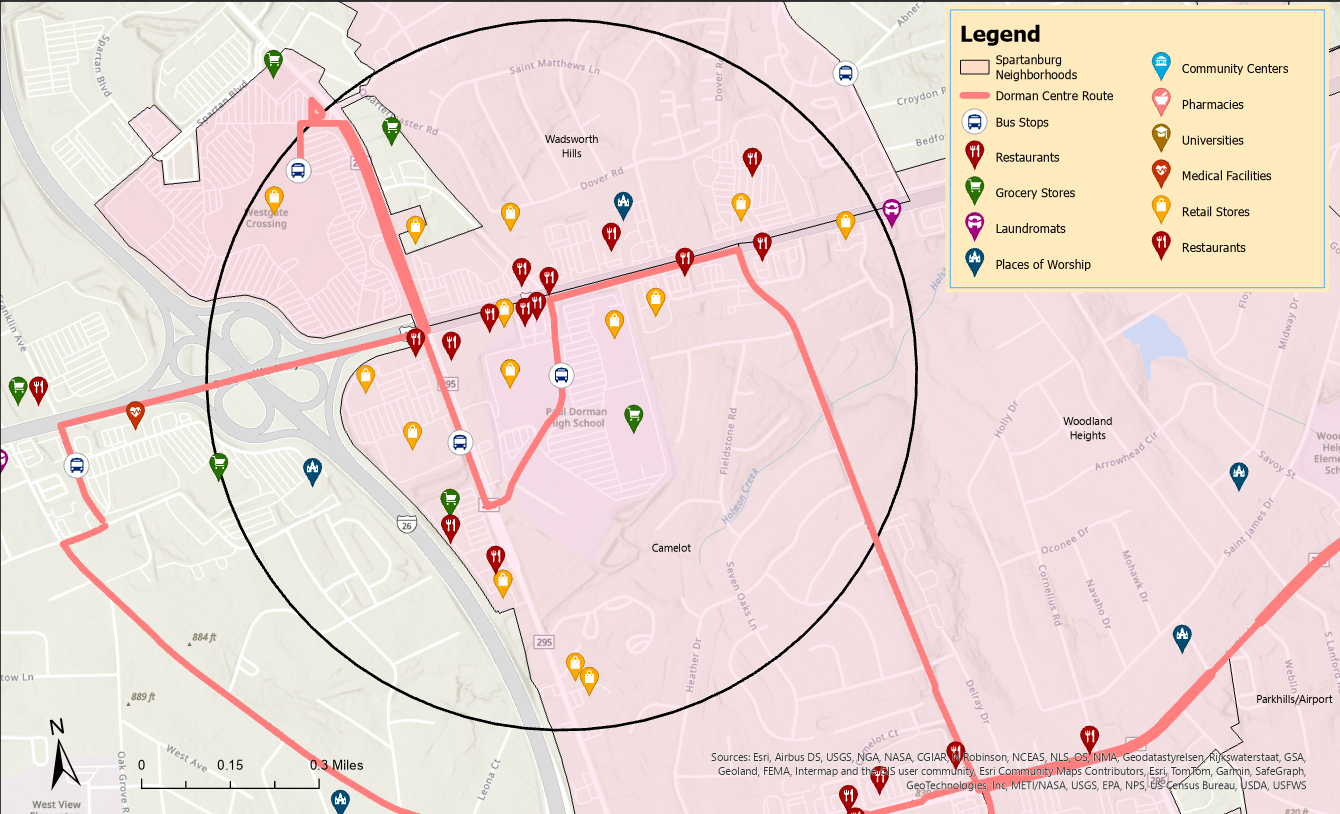
\includegraphics[width=1\linewidth]{dorman center best route.png}
    \caption {Dorman Center Inbound Stop}
    \label{fig:enter-label}
\end{figure}

\begin{figure}[ht]
    \centering
    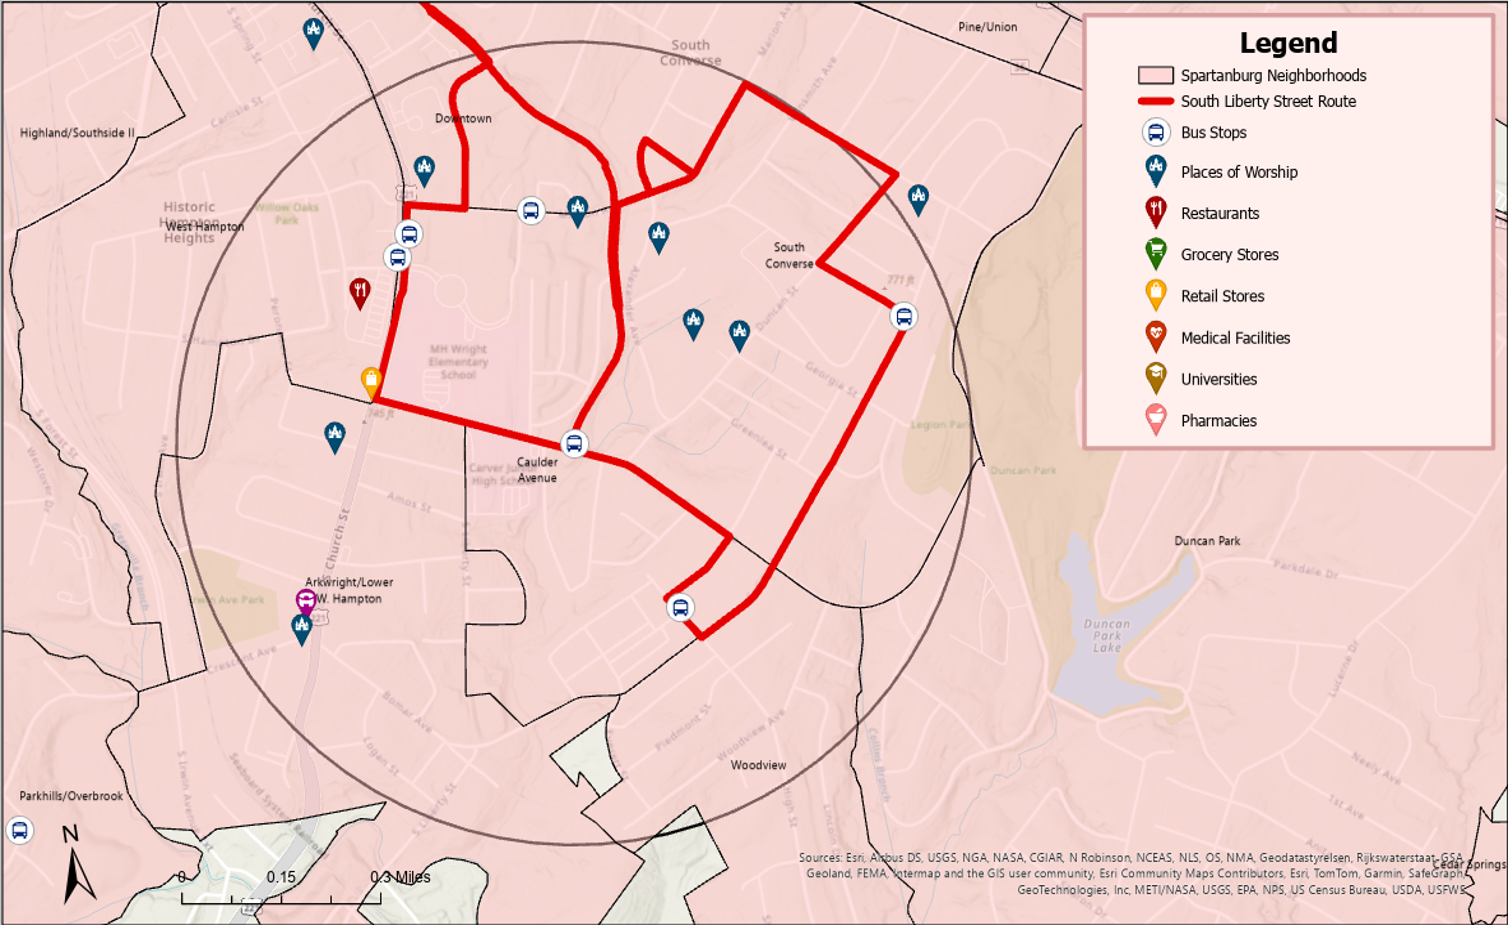
\includegraphics[width=1\linewidth]{libertystop.png}
    \caption {South Liberty Inbound Stop}
    \label{fig:enter-label}
\end{figure}

As previously stated, we were able to fully apply our model to two existing stops in the Spartanburg bus system: Dorman Center Stop 2 Inbound and South Liberty Stop 2 Inbound. The Dorman Center Inbound stop (see Figure 1) is in the center of one of the most dense shopping districts in all of Spartaburg. The 0.6 mile radius around this stop reaches a Walmart Supercenter, several major retail stores such as Ross and Best Buy, as well as part of the local shopping mall.

Within the 0.6 mile radius surrounding this stop, there exists at least one grocery store, three medical facilities, two places of worship, fourteen retail stores, and thirteen restaurants. Plugging this information into our model, we get that this bus stop has an accessibility score P = 10 + 5(3) + 4(2) + 2(14) + 13 = 74. 

The South Liberty Inbound stop (see Figure 2) is in the heart of a large residential district in southern Spartanburg, but still has a considerable amount of important services surrounding it. Within the 0.6 mile radius surrounding this stop, there exists seven places of worship, one laundromat, one retail store, one community center, and one restaurant. Plugging this information into our model, we get that this bus stop has an accessibility score P = 4(7) + 3(1) + 2(1) +2(1) + 1 = 36.

\subsection{Partial Model Application on Four Additional Bus Stops}

We were given additional map data that each have every current bus stop marked, with a corresponding 0.6 mile radius circle drawn around it. Figure 3 has every grocery store in Spartanburg plotted, while Figures 4 and 5 have every pharmacy and medical facility plotted, respectively. Using this data, we were able to apply the limited version of our model to four additional bus stops in the existing system: Crestview Stop 2 Inbound, Hillcrest Stop 2 Outbound, North Church Stop 3 Outbound, and Hillcrest Stop 2 Inbound.

The first two stops that we applied to our simplified model are ones that could be considered average to below average in the context of services and amenities. The Crestview stop lies in a heavily residential district near downtown Spartanburg, and does not have any grocery stores, medical facilities, or pharmacies in the 0.6 mile radius surrounding it. So, though it may provide a solid option for residents to get to the bus, it receives a simplified accessibility score P = 0. The Hillcrest Outbound stop, while lying along a major road that feeds into and out of downtown Spartanburg, is still largely surrounding by residential areas. The 0.6 mile radius around this stop has one grocery store and one medical facility within it, giving a simplified accessibility score P = 10 + 5(1) = 15. 

The latter stops are ones that lie in much denser shopping areas, similarly to the Dorman Center stop. The North Church Outbound stop lies next to a major medical complex as well as several businesses just north of Spartanburg. The 0.6 mile radius around this stop has one grocery store, six medical facilities, and five pharmacies within it. Thus, this stop receives a simplified accessibility score P = 10 + 9 + 5(6) = 49. Lastly, the Hillcrest Inbound stop lies right in the middle of the densest shopping district in eastern Spartanburg. The 0.6 mile radius around this stop has four grocery stores, four pharmacies, and one medical facility within it, giving it a simplified accessibility score P = 10 + 9 + 5(1) = 24.


\begin{figure}
    \centering
    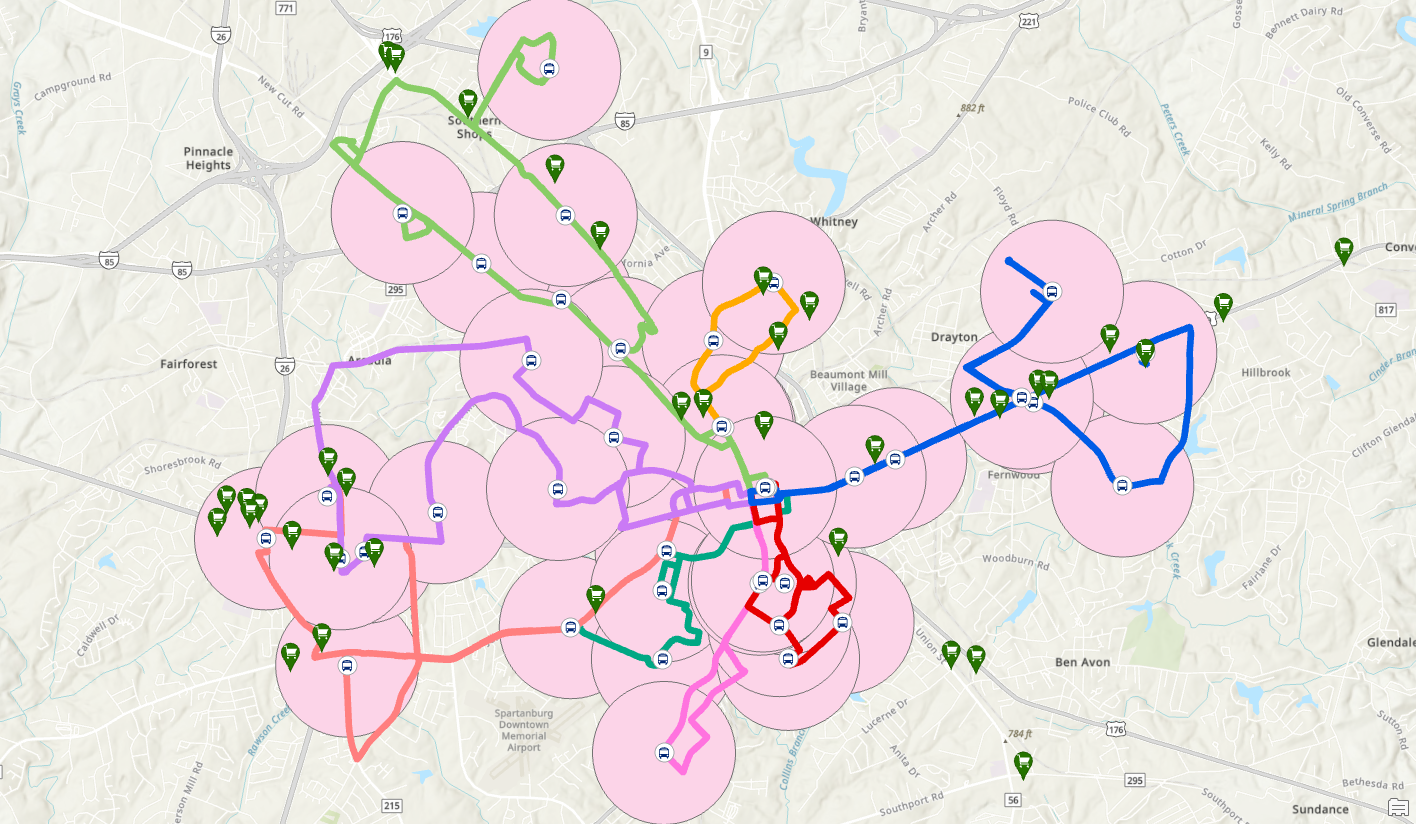
\includegraphics[width=1\linewidth]{groceries_bystop.png}
    \caption{Grocery Stores Along Bus Routes}
    \label{fig:enter-label}
\end{figure}
\begin{figure}
    \centering
    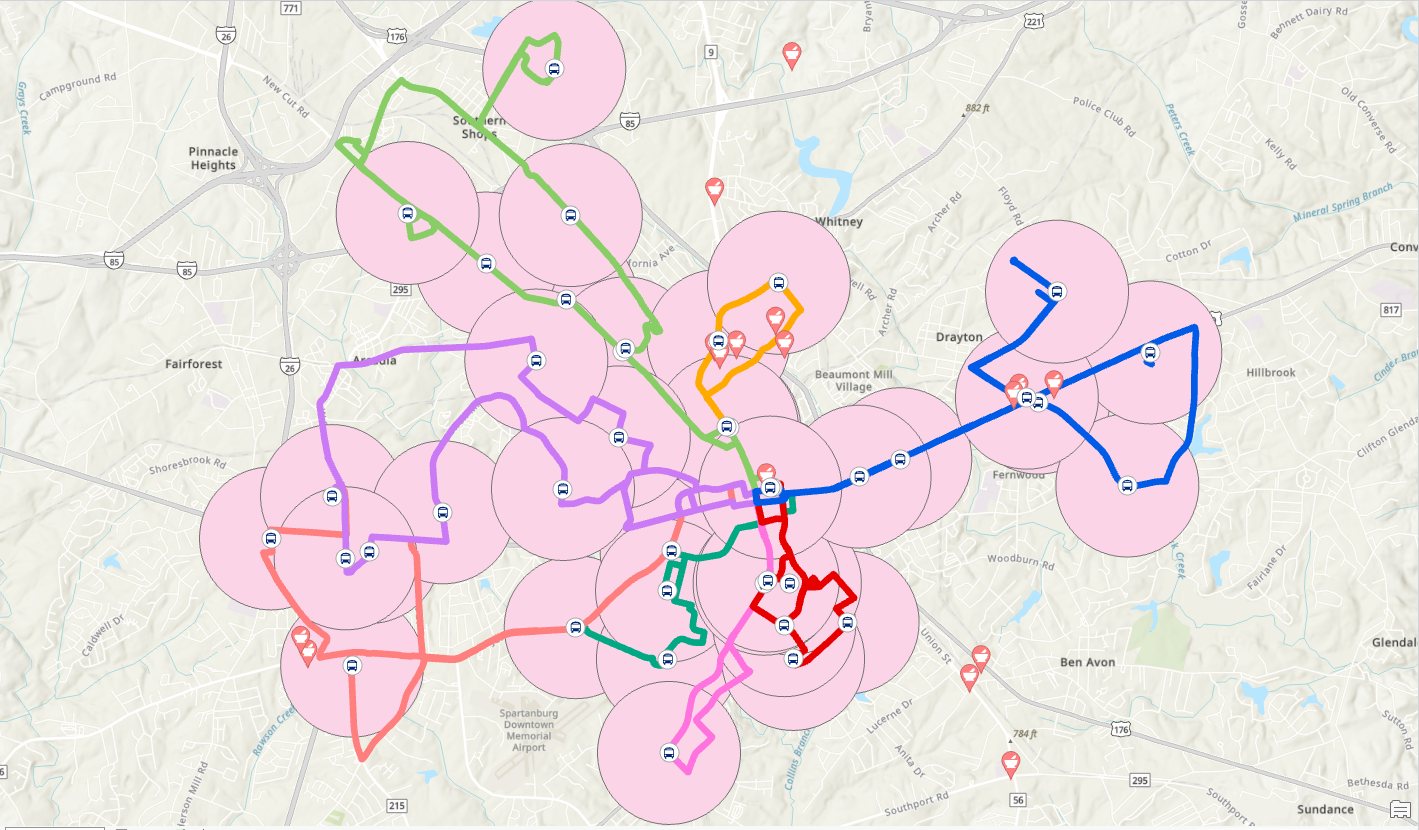
\includegraphics[width=1\linewidth]{pharmacies_bystop.png}
    \caption{Pharmacies Along Bus Routes}
    \label{fig:enter-label}
\end{figure}
\begin{figure}
    \centering
    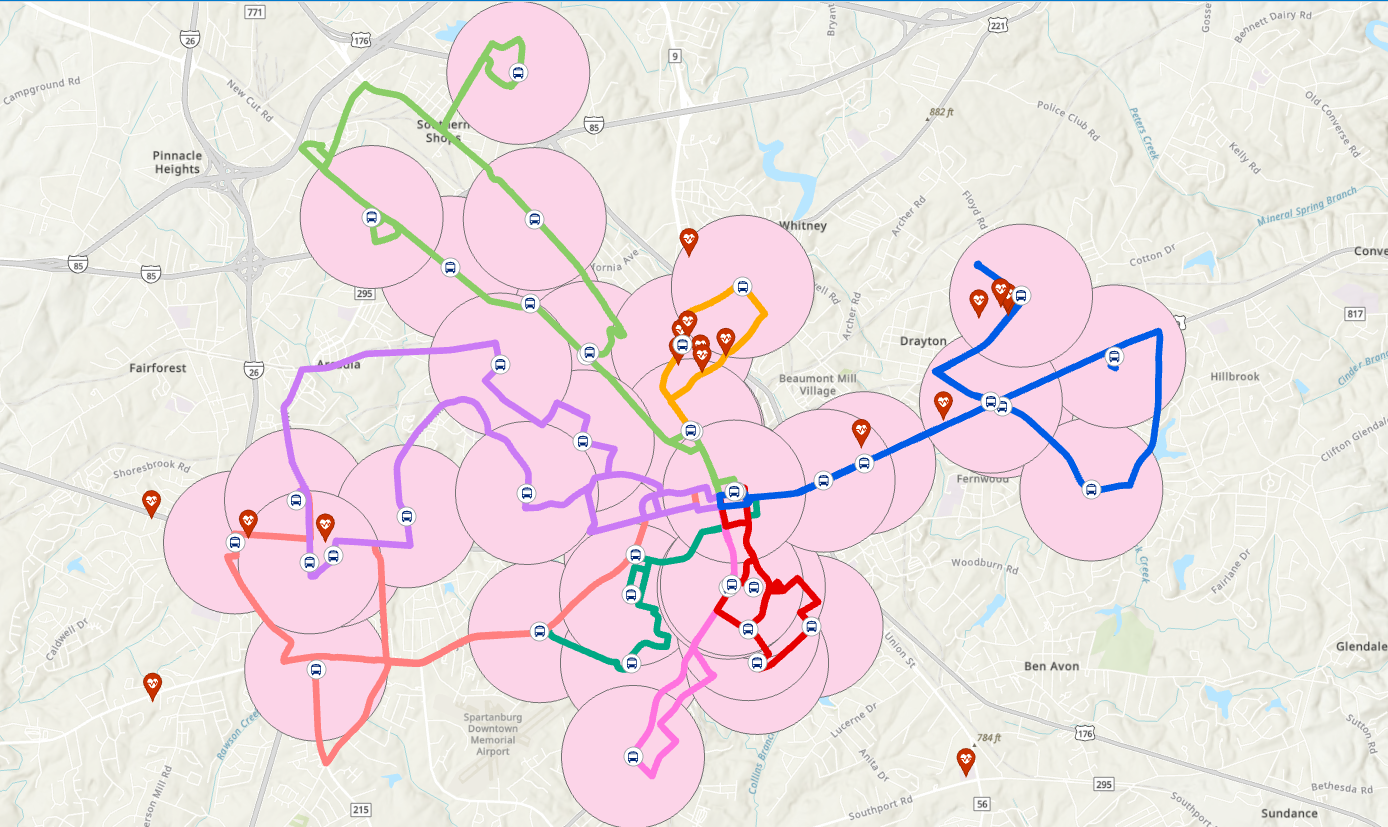
\includegraphics[width=1\linewidth]{medfacilities_bystop.png}
    \caption{Medical Facilities Along Bus Routes}
    \label{fig:enter-label}
\end{figure}


\subsection{General Analysis}

After analyzing our results, we feel that we were able to create a model that accurately assesses accessibility to services and amenities within the Spartanburg community. For the two stops we selected to fully apply our model to, we intentionally picked a heavily commercial stop and a heavily residential stop to see if our model outputted a drastic difference like we would expect. The Dorman Center stop received an accessibility score that is just over double that of the South Liberty stop, which reflects what we were expecting. In addition to this, the residential stops that we evaluated with the simplified model, Crestview and Hillcrest Outbound, received very low scores (0 and 15 respectively). This was expected, as we feel it is much more likely for a heavily residential area to have the smaller, less important services such as laundromats, churches, and restaurants than having the major services and amenities. Conversely, the more dense stops we evaluated, North Church and Hillcrest Inbound, recevied very respectable stores despite the limited amount of services assessed (49 and 24 respectively). In fact, the North Church stop received a higher score than the South Liberty stop, despite only evaluating the top three services for North Church and applying the entire model for South Liberty. We feel that this result further shows that our model appropriately assesses accessibility, by giving high scores to stops with a plentiful amount of services and giving low scores to stops in largely residential areas.



\subsection{Sensitivity Analysis}

We evaluated the accessibility of the bus stops by looking at our three highest-ranking amenities:  grocery stores, pharmacies, and medical facilities.  The same accessibility score weights and radius size surrounding the bus stops were used, with 10 points being given for the presence of at least one grocery store, 9 points for near a pharmacy, and 5 points for each medical facility.  When comparing the Dorman Center stop with the South Liberty stop, the Dorman Center stop’s score is significantly higher than the South Liberty stop.  The Dorman Center, having four grocery stores and three medical facilities earns 25 points from our accessibility score while the South Liberty stop does not contain any of the three services and amenities listed above and has a total of 0 from our accessibility score.  Therefore, examining only these three amenities in comparing Dorman Center stop and the South Liberty stop does not change the ranking of accessibility scores between the two stops.  Because focusing on these three categories does not change the ranking of these two stops based on accessibility scores, it is reasonable to view only these three categories in determining the accessibility scores.  
